% ============================================
% 数据结构模板 (Data Structure Templates)
% 适用：内存布局、指针关系、链表、数组
% ============================================

% --------------------------------------------
% 内存布局图（栈与堆）
% --------------------------------------------
\begin{figure}[H]
  \centering
  \begin{tikzpicture}
    % 栈区
    \draw[thick] (0,0) rectangle (2,3);
    \node at (1,3.3) {栈 (Stack)};
    \draw (0,2.5) -- (2,2.5);
    \draw (0,2.0) -- (2,2.0);
    \draw (0,1.5) -- (2,1.5);
    \node at (1,2.75) {\small 局部变量1};
    \node at (1,2.25) {\small 局部变量2};
    
    % 堆区
    \draw[thick] (4,0) rectangle (6,3);
    \node at (5,3.3) {堆 (Heap)};
    \node at (5,1.5) {\small 动态分配};
    
    % 指针箭头
    \draw[->, thick] (2.1,2.25) -- (3.9,1.5);
  \end{tikzpicture}
  \caption{栈与堆的内存布局}
  \label{fig:memory_layout}
\end{figure}

% --------------------------------------------
% 指针指向图
% --------------------------------------------
\begin{figure}[H]
  \centering
  \begin{tikzpicture}[
    box/.style={draw, rectangle, minimum width=1.5cm, minimum height=0.8cm},
    label/.style={font=\small}
  ]
    \node[box] (ptr) at (0,0) {0x1000};
    \node[label, above=0.1cm of ptr] {p (指针)};
    
    \node[box] (var) at (4,0) {42};
    \node[label, above=0.1cm of var] {value};
    \node[label, below=0.1cm of var] {\tiny 地址: 0x1000};
    
    \draw[->, thick] (ptr.east) -- (var.west);
  \end{tikzpicture}
  \caption{指针 p 指向变量 value}
  \label{fig:pointer_ref}
\end{figure}

% --------------------------------------------
% 链表结构
% --------------------------------------------
\begin{figure}[H]
  \centering
  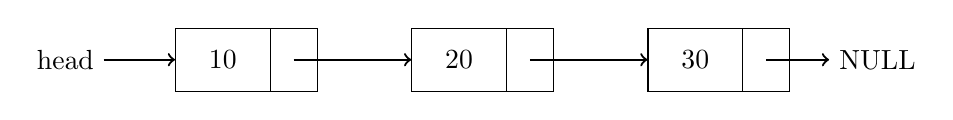
\begin{tikzpicture}[
    node/.style={draw, rectangle, minimum width=1.2cm, minimum height=0.8cm},
    ptr/.style={draw, rectangle, minimum width=0.6cm, minimum height=0.8cm}
  ]
    % 节点1
    \node[node] (n1) at (0,0) {10};
    \node[ptr] (p1) at (0.9,0) {};
    
    % 节点2
    \node[node] (n2) at (3,0) {20};
    \node[ptr] (p2) at (3.9,0) {};
    
    % 节点3
    \node[node] (n3) at (6,0) {30};
    \node[ptr] (p3) at (6.9,0) {};
    
    % 连接箭头
    \draw[->, thick] (p1.center) -- (n2.west);
    \draw[->, thick] (p2.center) -- (n3.west);
    \draw[->, thick] (p3.center) -- ++(0.8,0) node[right] {NULL};
    
    % head 指针
    \node (head) at (-2,0) {head};
    \draw[->, thick] (head.east) -- (n1.west);
  \end{tikzpicture}
  \caption{单向链表结构}
  \label{fig:linked_list}
\end{figure}

% --------------------------------------------
% 数组内存视图
% --------------------------------------------
\begin{figure}[H]
  \centering
  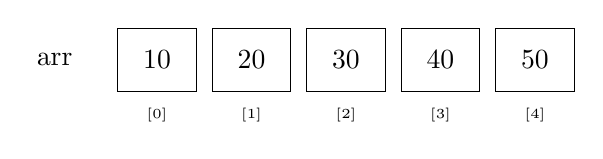
\begin{tikzpicture}
    \foreach \i/\v in {0/10, 1/20, 2/30, 3/40, 4/50} {
      \draw (\i*1.2, 0) rectangle (\i*1.2+1, 0.8);
      \node at (\i*1.2+0.5, 0.4) {\v};
      \node at (\i*1.2+0.5, -0.3) {\tiny [\i]};
    }
    \node at (-0.8, 0.4) {arr};
  \end{tikzpicture}
  \caption{数组 arr 的内存布局}
  \label{fig:array_memory}
\end{figure}
